\documentclass[11.5pt]{sig-alternate} % sets document style to sig-alternate
% packages
% typesetting
%\usepackage{dirtytalk} % typset quotations easier (\say{stuff})
\usepackage{hanging} % hanging paragraphs
\usepackage[defaultlines=3,all]{nowidow} % avoid widows
\usepackage[pdfpagelabels=false]{hyperref} % produce hypertext links, includes backref and nameref
\usepackage{xurl} % defines url linebreaks, loads url package
\usepackage{microtype}
\usepackage{textgreek}
%\usepackage{textcomp}
%\newcommand{\texttildemid}{\raisebox{0.4ex}{\texttildelow}}
% layout
\usepackage{enumitem} % control layout of itemize, enumerate, description
\usepackage{fancyhdr} % control page headers and footers
\usepackage{float} % improved interface for floating objects
%\usepackage{multicol} % intermix single and multiple column pages
% language
\usepackage[utf8]{inputenc} % accept different input encodings
\usepackage[english]{babel} % multilanguage support
% misc
\usepackage{graphicx} % builds upon graphics package, \includegraphics
%\usepackage{lastpage} % reference number of pages
%\usepackage{comment} % exclude portions of text (?)
\usepackage{xcolor} % color extensions
\usepackage[backend=biber, style=apa]{biblatex} % sophisticated bibliographies % necessary for HTML to display author info and date on abstract page
\usepackage{csquotes} % advanced quotations, makes biblatex happy
\usepackage{authblk} % support for footnote style author/affiliation
% tables and figures
\usepackage{tabularray}
%\usepackage{array} % extend array and tabular environments
\usepackage{caption} % customize captions in figures and tables (rotating captions, sideways captions, etc)
%\usepackage{cuted} % allow mixing of \onecolumn and \twocolumn on same page
\usepackage{multirow} % create tabular cells spanning multiple rows
%\usepackage{subfigure} % deprecated, support for manipulation of small figures
%\usepackage{tabularx} % extension of tabular with column designator "x", creates paragraph-like column whose width automatically expands
%\usepackage{wrapfig} % allows figures or tables to have text wrapped around them
%\usepackage{booktabs} % better rules
% dummy text
%\usepackage{blindtext} % blind text dummy text
%\usepackage{kantlipsum} % Kant style dummy text
\usepackage{lipsum} %lorem ipsum dummy text
% other helpful packages may be booktabs, longtable, longtabu, microtype

\pagestyle{fancy} % sets pagestyle to fancy for fancy headers and footers

% header and footer
% modern way to set header image
\renewcommand{\headrulewidth}{0pt} % defines thickness of line under header
\renewcommand{\footrulewidth}{0pt} % defines thickness of line above header
\setlength\headheight{80.0pt} % sets height between top margin and header image, effectively moves page contents down
\addtolength{\textheight}{-80.0pt} % seems to affect the lower height. maybe only works properly if footer numbers enabled?
\fancyhf{}
\fancyhead[CE, CO]{
\includegraphics[width=\textwidth]{headerImage.png}}
% footer
%\fancyfoot[LE,LO]{Article Title Here \\ DOI: }% left footer article title and doi
%\fancyfoot[CE,CO]{{}} % center footer empty
%\fancyfoot[RE,RO]{\thepage} % right footer page numbers
%\pagenumbering{arabic} % arabic (1, 2, 3) numbering in footer

\hypersetup{colorlinks=true,urlcolor=blue} % sets link color to blue
\urlstyle{same} % sets url typeface to same as rest of text

% set caption and figure to italics, label bold, left align captions, does not transfer to HTML
\captionsetup{labelfont=bf, font={large, it}, justification=raggedright, singlelinecheck=false}
\renewcommand\theContinuedFloat{\alph{ContinuedFloat}}

%this next bit is confusing, but essentially changes the width of the abstract. Seems to have been copied from this https://tex.stackexchange.com/questions/151583/how-to-adjust-the-width-of-abstract
\let\oldabstract\abstract
\let\oldendabstract\endabstract
\makeatletter %changes @ catcode to enable modification (in parsep)
\renewenvironment{abstract} %alters the abstract environment
{\renewenvironment{quotation}%
               {\list{}{\addtolength{\leftmargin}{1em} % change this value to add or remove length to the the default ?
                        \listparindent 1.5em%
                        \itemindent    \listparindent%
                        \rightmargin   \leftmargin%
                        \parsep        \z@ \@plus\p@}%
                \item\relax}%
               {\endlist}%
\oldabstract}
{\oldendabstract}
\makeatother %changes @ catcode to disable modification

% checks
% italics
% links
% dashes
% tildes
\begin{document}

\title{Development of a Curriculum to Teach the “Soft Skills” Necessary for the Future Deaf and Hard-of-Hearing Laboratory Technician Workforce}

\author[1]{\large \color{blue}Annemarie D. Ross}
\author[1]{\large \color{blue}Todd Pagano}

\affil[1]{Rochester Institute of Technology/National Technical Institute for the Deaf}

\toappear{ }
%% ABSTRACT
\maketitle
\begin{@twocolumnfalse} 
\begin{abstract}
\item 
\textit{There is often a particular void in the education of deaf and hard-of-hearing students who intend to become competent working laboratory technicians. Inasmuch as certain basic professional skills (“soft skills”, in this case) are not generally taught in traditional science courses, a new curriculum has been developed in order to enforce these skills. The “soft skills” of focus in this study are safety awareness, technical writing, and teamwork/conflict resolution. The development of the pedagogical tools used to teach these specific “soft skills” are discussed, as well as an assessment of the augmentation in student understanding in each skill area. By incorporating an interdisciplinary approach that enforces “soft skills”, students should find greater success while on co-operative work experiences and have more prominent career opportunities. This curriculum was produced for the Chemical Technology-like program, Laboratory Science Technology, at the National Technical Institute for the Deaf- one of the eight colleges of the Rochester Institute of Technology, but the concepts are transferable to other technical-based programs.}
\\ \\ 
\end{abstract}
\end{@twocolumnfalse}

%% AUTHOR INFORMATION

\textbf{*Corresponding Author, Annemarie D. Ross} \\
\href{mailto:adrnts@rit.edu}{(adrnts@rit.edu)} \\
\textit{Submitted  Apr 14 2014} \\
\textit{Accepted Apr 14 2014} \\
\textit{Published online Apr 14 2014} \\
\textit{DOI:10.14448/jsesd.02.0003} \\
\pagebreak
\clearpage
\begin{large}
\section*{INTRODUCTION}

“Soft skills” are necessary for inclusion in the Chemical Technology (sometimes referred to as Applied Chemistry) or Laboratory Science curriculum because they relate to important topics that can impact not only the program’s graduates, but everyone in their shared laboratory environment. These “soft skills”; which include (to name a few) material safety data sheets (MSDS) documentation and other safety-related knowledge, technical writing skills, and the ability to work as a member of a team are often not fully emphasized within a program’s traditional coursework. These “soft skills” may be especially important for deaf and hard-of-hearing programs, as attempts are to give these students every possible competitive advantage as they will naturally face communication and other barriers. Graduates will need a strong foundation in “soft skills” to help foster their success in the field.

A former student in a cooperative work experience (co-op)/internship position had the awkward moment of not knowing how to look up information in an MSDS for a specific chemical. This is a crucial skill that is not only necessary for the chemical technician, but is also a safety risk to the student, as well as to those working in the shared laboratory environment. This problem might not have occurred if this skill was directly taught in the student’s college preparatory coursework.

The overwhelming focus of most scientific courses tends to be on the inherent technical content. This unfortunate occurrence of some two-year programs’ focus on technical content while minimizing attention to “soft skills” has been reported as a subset of “employability skills”, such as communication skills, by the American Chemical Society’s (ACS) National Science Foundation (NSF) sponsored program, ChemTechLinks (American Chemical Society, 2006).

Though mastery of technical content is critical, industry looks for candidates who have applied skills along with knowledge of “soft skills”- like working in a team environment and ensuring quality control while being able to effectively communicate results (Kalivas, 2005). However, as Kalivas (2005) goes on to recognize, college graduates are often lacking these desired skills. It is widely supported that Chemical Technology students who learn and master “soft skills” will become desired graduates by employers (DeWitt, 2008). 

Academic programs, especially vocational and two-year degree programs, need to make sure that they are producing the graduates that industry desires. To this end, experts have indicated that Chemical Technology programs are often more successful if they include industrial-partner influenced curricula to acquire their perspective on required skills for competent technicians (Aronson and Wesemann, 2007). This need for skilled graduates is further supported by the manufacturing industry, for which 90\% of polled companies are finding it difficult to hire skilled technicians according to a National Association of Manufacturers survey (HennessyFiske, 2006). One tool that begins to address the need to align academia with industry’s needs is the ChemTechStandards database (formerly called the Voluntary Industry Skills Standards database) developed by the ACS, in order to prioritize various skills required for success in the field, including “soft skills” (the database can be found at \url{https://portal.acs.org/portal/acs/corg/coldfusionapp?_nfpb=true&_pageLabel=mapp_cts_page}–accessed June, 2009). Skill standards based on industry’s needs are important in training students to be ready for the workforce, as they are found in industry-desired skills (Davis, 2006). 

The ACS and NSF have a history of supporting curriculum development projects, including the Contextual Laboratory Curriculum for Chemistry and Technology (C3T) program (White, 2004). Through this project, investigators developed competency-based modules that apply directly to the ACS ChemTechStandards data-base and inherent “soft skills”. One example is the “Communicating Results” module which includes how to keep a good laboratory notebook during laboratory experimentation and how to clearly present technical results.

The successes of industry-academia partnerships have been illustrated in the case of seven industrial plant managers taking action and collaborating with the College of Mainland (Texas) to develop a two-year Associate of Applied Science degree (AAS) in Process Technology (Payne \& Williams-Foster, 1997). This degree was established in 1994, after both the college and the plant representatives developed the curriculum by serving on an advisory committee together. The reports states that three years later, significant funds were saved by the company since basic training days were reduced by a remarkable 68\% at an estimated \$40,500 savings in cost (Payne \& Williams-Foster, 1997).

The Laboratory Science Technology (LST) program at the National Technical Institute for the Deaf (NTID) is an Associate degree level program that often places its graduates directly into industry and requires a co-op experience for graduation. The program is an ACS Chemical Technology Program Approval Service (CTPAS) approved program, and about 25 deaf and hard-of-hearing students enter this Chemical Technology-like program every year. The program focuses on the applied knowledge that graduates need in order to “hit the ground running” when they arrive at their co-op site or place of employment. It is the philosophy of the LST program to give its students every possible competitive advantage when they enter the workforce. 

The deaf and hard-of-hearing students of the LST program enter their co-ops and careers with strong hands-on experience, and students should be confident that they are ready to handle many situations that might arise in the laboratory setting. During co-op experiences, conflict resolution issues have arisen between students and co-workers which required professors of the LST program to relate “soft skills” in the program’s curriculum (Pagano \& Quinsland, 2007). With the proposed curricular modifications, topics can be taught so that students will have an additional advantage because their detailed familiarity with the “soft skills” will complement their high-level applied technical skills. 

Technical writing is a “soft skill” that is a common point-of-weakness with new employees as they enter the workforce. Jean Lummis (2001), a newly graduated chemist at the time, took a job at the Food and Drug Administration only to find that she (in addition to others in her department) had such a lack of technical writing training that they were sent to a workshop to improve their skills. As a result, she decided to incorporate technical writing into her classroom when she began a teaching career (Lummis, 2001). Others further support the need to teach writing because technical employees may not have enough experience in the writing of various types of reporting documents (Kennedy, 2004). Technical writing is especially important for deaf and hard-of-hearing individuals since English can be a second language for many students, so writing, in general, can be a challenge.

In addition to teaching technical writing skills, educators are incorporating lessons in teamwork. An NSF white paper (Stander, 2000) reported a study on Chemical Technology students and their personality types in order to better understand what type of learners tend to comprise these programs. This report is useful because it provides insight as to what type of personalities might work well in a team setting and how students can use the knowledge of their own personality types to address conflicts as they work in teams. The findings reported that national Chemical Technology students are I/ESTJ (I and E are almost equal in percentage at 51\% and 49\% respectively); where I = Introvert, E = Extrovert, S= Sensing, T = Thinking, and J = Judging (other possibilities are N = Intuitive, F = Feeling, and P = Perceiving) (Stander, 2000). Individuals with this particular personality type tend to “think” and “judge”, which requires a certain structure as they approach tasks (Stander, 2000). This information can be used to begin thinking about mechanisms for teaching teamwork-related topics.

\section*{METHODS}

As previously stated, there are many different “soft skills” that are required of chemical technicians, but the following subset was chosen for the confines of this study: MSDS/safety, technical writing, and teamwork/conflict resolution. These “soft skills” are shown in Figure 1, and were chosen based on the importance of what basic skills are needed for student success, as well as the “soft skills” that are important to the deaf and hard-of-hearing professional’s work environment.

\begin{figure}[h]
    \centering
    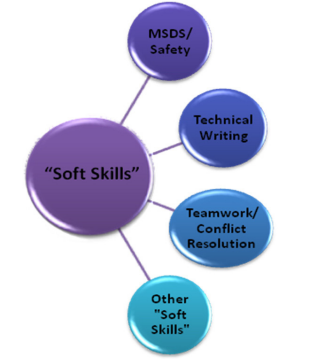
\includegraphics[width=1\linewidth]{images/fig1.png}
    \caption{“Soft Skills” examined in this study: MSDS/Safety, Technical Writing, and Teamwork/Conflict Resolution. }
\end{figure}

In addition to selecting “soft skills” for inclusion, the development of the course modifications involved determining the goals and objectives of the course- which are based on Bloom’s Taxonomy and the following six inherent general categories: knowledge, comprehension, application, analysis, synthesis, and evaluation (Bloom, 1956). Using these general categories, objectives are specifically stated for each “soft skill” topic along with strategies to satisfy each stated objective. Keeping cognitive levels in mind, familiarity with the LST curriculum was required in order to see where in the course timeline modifications would belong. 

As course materials were developed, careful attention was given to the future assessment of  designed lesson plans. In general, the assessment technique was determined based on what the students are expected to know before the lesson plan in order to perform pre-/post- assessments. This was especially important in the MSDS assessment since students were not expected to be familiar with MSDS prior to the lesson. To this end, a pre-assessment could not take place such as that done in the technical writing assessment. Therefore, the proper assessment was done by evaluating questions on exams that pertained to the MSDS topic, after the skills were taught.

The MSDS/safety materials were taught in the Laboratory Applications I (0879-201) course with the first year LST students since the material is of critical importance for working in even an academic laboratory, and foundation knowledge is needed for subsequent coursework. The teamwork and the technical writing lessons were taught in Chemical Technology (0879-313), a course with second-year LST students who had already experienced intensive teamwork situations in the laboratory and have had plenty of writing assignments. This timely information is being reinforced to students just prior to their required co-op assignment. To better accommodate the deaf and hard-of-hearing students in the program, the Keirsey Temperament Sorter was given to discover their four letter code (personality type) instead of the Myers-Briggs assessment. Keirsey adapted his method to that of “JungMeyers typology”, (Myers being that of Isabel Briggs Myers who co-developed the MyersBriggs type indicator with her mother, Katharine Cook Briggs) to include their “concepts of type” (Keirsey \& Gates, 1984) cal writing activity by comparing pre- and post-memo assignments. For MSDS/safety, the assessment is based on exam results from questions specific to the MSDS topic. And for teamwork/conflict resolution, the analysis is on the comparison of the personality type of the current second-year LST students to the reported national Chemical Technology student Myers-Briggs type from the NSF white paper (Stander, 2000). Current student success can only be measured in present time, while we wait a few years to see the true measurement of student success in the work environment based on these implementations (an ultimate goal of this project). As such, a full assessment of the aims of this project is outside its current scope and the results here are of immediate/preliminary nature

\section*{Results}
The developed curriculum is heavily based on Bloom’s Taxonomy in order to make sure that the content matched student cognitive levels and covered the important aspects of what the students needed to learn in the area of “soft skills”. The basic six categories represent a building pattern of knowledge, and is a measurement of how readily students grasp a concept. Each category is a level of understanding, which starts at recalling information and continues to the ability to evaluate information so that students can make their own unique judgments about that information. This is heavily based on students’ cognitive abilities during various stages of the learning process. The six general categories were addressed and documented for every lesson plan developed. A general visual representation of the timelines for the developed lesson plans is shown in \textbf{Figure 2}
\newpage
\begin{figure}[h]
    \centering
    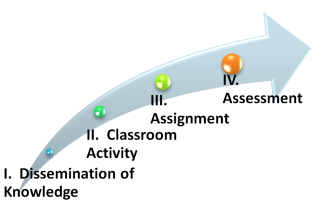
\includegraphics[width=1\linewidth]{images/fig2.png}
    \caption{General timeline for the development of lesson plans on each “soft skill”- in four basic steps: Dissemination of Knowledge, Classroom Activity, Assignment, and Assessment.}
\end{figure}

\subsection*{MSDS/Safety}

The first lesson taught was related to MSDS/safety, which began with a lecture to explain the various components of a typical MSDS. Since MSDS sheets are safety tools for which students must be familiar, the goal of the lesson was for the students to have a detailed understanding of what each section of the MSDS tells the user, and if they need to find certain information, where in the MSDS it would be found. It is imperative that students prove mastery of this crucial topic. During the lecture, a detailed handout was provided with a description of each section, along with a sample MSDS. While referring to these handouts during the lecture, students were asked to find specific information, such as the melting point of assigned chemicals, so that it could be assessed if the students understood how to use that section of the MSDS.

After the lecture, an in-class team activity was performed using a worksheet where the students were asked to use online MSDS databases to find specific information about various chemicals. For added incentive, the students were required to find the information to earn bonus points, based on accuracy and how quickly they completed the worksheet. During the activity, the students were able to ask for help in situations where terminology needed to be explained, and if they struggled to find information, hints were provided. At the end of the class activity, the students were given an assignment to find an MSDS for a given chemical and to answer the questions on an assignment sheet, using the MSDS.

The MSDS topic was concluded with an inclass exam two weeks after the class activity, to provide them with one week to complete their assignment, and the second week to receive feedback on their assignment, then to study for the exam. Prior to teaching the MSDS topic, it was decided that a preassessment would not be useful in this situation, since an assumption would have to be made that the students had prior knowledge of MSDS. The purpose of this lesson was to introduce the MSDS tool to students who had no prior knowledge, so the MSDS-related questions that were on the cumulative final exam were analyzed as a form of assessment. The class average on the MSDS questions of the final exam was 94.2\% (n=22), which reflects a strong score. It is acknowledged that the assessment in this instance may be terse, but more extensive activities and assessment are planned for future studies. 

During activities, it was observed that the handouts were beneficial to keep the students engaged and to incorporate an active hands-on learning activity. The in-class team activity proved to be a successful technique since the students had fun “competing” with each other, while becoming familiar with using the MSDS resources. Students also learned important new terminology with which they were not familiar.

\subsection*{Technical Writing}

In the technical writing lesson, students were first given an assignment to write a memo based on their laboratory experimental results and to turn it in during the next class session. These memos were collected for a pre-assessment of student abilities in writing memos. At the next class, it was announced that they were to rewrite their memos based on what would be covered in the lecture on that day, and to turn this second pass memo in as a postassessment of student abilities. The intermediate technical writing lesson involved a lecture explaining the sections of a memo and its technical format by showing visual examples of a professional memos. During the class period, an activity where students worked in teams involved a memo that was cut-up into pieces, and was then provided for the teams to re-assemble in a way that they believed would represent a strong professional memo. When the team activity was complete, they compared their re-assembled memo to the correct memo format, and the lesson plan concluded with the post-memo assignment. For both the pre- and post- assessments, an outside faculty member graded the memos, while additional feedback was provided to the students on some technical aspects that they may not have fully understood during their first pass at the material. The involvement of the outside faculty member was also to avoid personal bias in grading. Student grades improved by at least one letter grade after the lesson activities, on average the student score improved from 77.7\% to 90.6\% from the pre- and post-lesson memo assessment (n=12). Again, more activities and assessment are planned for future studies.

One observation was that the students struggled a bit with the classroom activity, but (mostly) understood the concept of the flow and format of a professional memo. Based on the assessment, it seems that students substantially improved their memo writing technique and will hopefully reflect back to the activity when they encounter future situations where they are required to write a memo on the job or co-op/internship.

\subsection*{Teamwork/Conflict Resolution}

Based on observations of student interaction in the laboratory and classroom environment, it was noticed that many conflicts arise in team settings due to attitudinal and personality differences. Thus, in addition to promoting teamwork into the class activities (like that in the technical writing lesson plan), it was realized that it would be of benefit to these students if they were aware of the different types of personalities that they might encounter in the future, as well as understanding their own personality types. If they become aware of personality types, they might use this information to try and better understand how to resolve an issue with a person of similar or opposite personality type within a collaborative setting.

The lesson plan consisted of opening a dialogue to discuss the teamwork conflicts that they have personally experienced, leading into completion of the Keirsey Temperament Sorter survey. They compared their types to their classroom peers, and a discussion ensued based on how the simple fact of a different personality can cause conflicts. The students were also asked to read the Keirsey Temperament Sorter personality descriptions and discuss if they believed that it was an accurate reflection of their individual personality.

\begin{figure*}[th]
    \centering
    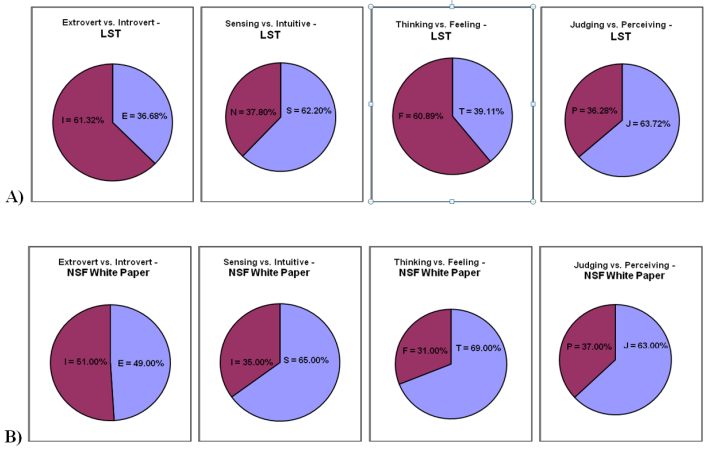
\includegraphics[width=1\textwidth]{images/fig3.png}
    \caption{A): Breakdown of Keirsey Temperament Sorter Personality Type indicators for second-year LST students- average LST student=ISFJ. B): Breakdown of Myers-Briggs Personality Type indicators for national Chemical Technology students reported in the NSF White Paper (Stander, 2000)- average national Chemical Technology student=I/ESTJ.}
\end{figure*}

Instead of an assessment of how the students worked in teams, their personality types were compared to the personality type of national Chemical Technology students that a study reported in a NSF white paper (Stander, 2000). In \textbf{Figure 3}, it is shown how the Laboratory Science Technology second-year students compare to the results in the NSF report. As can be seen, the average personality type for students in the LST program is ISFJ, which may mean that the program is attracting a slightly different type of Chemical Technology student than those of the NSF report.

% fig 3

As student reactions were observed during the personality discussion, they were surprised that the majority of them were in the ISFJ category, and thought that perhaps some conflicts arise because issues and confrontations are taken personally rather than objectively. Though the LST students appear to be a bit more introverted, the fact they likely analyze situations by “feeling” (rather than “thinking”) is the trait that might set them apart the most from the national average Chemical Technology student. This is probably the biggest lesson that was learned by students through this activity, since they realized that they must not bring their personal feelings into a profession al situation where they need to work together to accomplish a task.

\section*{DISCUSSION}

Industry depends on academia to provide quality employees to the workplace, so it is imperative that these academic programs listen to the needs of industry while educating students. Industry and academia are often inappropriately considered two different entities, but in reality have overlapping goals, specifically in the education of students/future technicians and in the teaching of “soft skills”. As shown in \textbf{Figure 4}, the importance of “soft skills” is essential in the “clockwork” of a Chemical Technology program. The “soft skills” serve as a mechanistic intermediate that allows the lifelong learning skills and technical content to work together and produce a more prominent chemical technician \\

\begin{figure}[h]
    \centering
    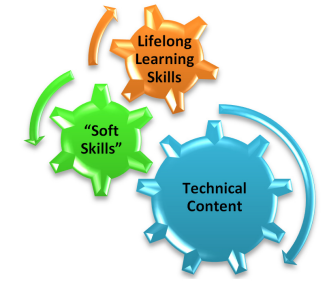
\includegraphics[width=1\linewidth]{images/fig4.png}
    \caption{The “clockwork of an academic program” in preparing chemical technicians}
\end{figure}

Past studies have documented that these skills are lacking, and now it is up to academia to ensure that our graduates are getting these “soft skills” and are ready to enter the workforce possessing a better skill-set for competitive positions. In effect, goals in industry and academia not only overlap, but can work together to make sure that graduates are getting the education that they need.

In order to fill the “soft skills” void in the curriculum, approaches were taken to turn it into a strength of the LST program. In the MSDS/ safety lesson activities, it was shown that the students average score was in the ‘A’ range on the MSDS specific questions of the exam. This score shows that the students have a good understanding of how to interpret MSDS and how to use it as a tool for their safety. By having students follow along during the lecture, and then apply their newly learned skill to their teamwork activity involving the use of resources to find information from MSDS, the lesson plan helped students to actively learn how the MSDS is a tool for safety. As such, the overall lesson plan was effective.

Technical writing was obviously a needed lesson for these students as they showed vast improvement on their pre- and post- lesson memo assignments. It is believed that the lesson developed for this skill was one that was effective based on the improvement in scores, as well as the observed improvement in the writing produced by the students throughout the remainder of their program. As can be seen along with the other two lesson plans, the success shows that it is highly effective to incorporate multiple modalities of teaching in order to reinforce the material in different ways and to reach all types of student learners. 

In the final lesson, the Keirsey Temperament Sorter questionnaire was provided to the students so that they could learn more about their own personality as well as that of their peers. They often work with their peers in the lab, and knowing their differences in personalities allowed them to reflect on why conflicts arise as they collaborate. This helped with conflict resolution since they understood that conflicts arise naturally, because when two or more people come together to approach a problem, they do so from different personality perspectives. In addition, it seems that an unexpected result was uncovered in that the NSF white paper (Stander, 2000) found a majority of I/ESTJ type for national Chemical Technology students, while the LST program has a majority of ISFJ personality type in the secondyear majors. It seems that the LST program is attracting a different group of chemical technicians; perhaps partially due to the fact our program is specific to the deaf and hard-of-hearing population. Variations in results of the Myers-Briggs and Keirsey Temperament Sorter could also limit the direct comparison of data

\section*{CONCLUSION}

This study involved the development of a detailed curriculum for the LST program to incorporate into its course mask, though the concept is also applicable to other programs. One obvious group of benefit may be those Chemical Technology/Applied Chemistry programs that may also be lacking such “soft skills” by using this curriculum as a starting point for modification according to their desired standards. In the long run, industry will experience improved efficacy as they hire graduates who already possess the requisite skills and do not require additional time to acquire these skills while on the job

The deaf and hard-of-hearing students of the LST program often need reinforcement in the area of “soft skills”, especially since barriers are already present as they interact with co-workers who may be unaware of communication issues. These students will likely already have enough challenges to face in the workforce due to these communication and attitudinal barriers pertaining to their deafness. The emphasis of teamwork/conflict resolution in the curriculum will help students gain confidence as they approach these barriers and acquire techniques to handle such situations. In effect, these “soft skills” will provide students with skills that will give them a competitive advantage as they search for jobs- by demonstrating their understanding and experience in “soft skills”, along with their technical degree, they should be more desired in the workplace.

In this study, it was found that incorporating different learning modalities to reinforce the lesson in multiple ways and involving active learning allowed the students to better retain the information. In addition, it was effective to include teamwork activities throughout the lessons so that students naturally learn how to work together and learn new techniques as some conflicts may arise as a function of collaboration. Since the program has a unique population of students who are deaf and hard-of-hearing, it was a challenge to see how the different communication preferences work together: American Sign Language (ASL) fluent students with oral students, non-ASL fluent cochlear implant students with ASL fluent students, and other variations. There were some issues related to students not working together, but instead working individually, as they had different communication preferences and skills. This issue was resolved by reinforcing their need to work together, which after several “pushes”, they eventually did. It seemed obvious that the students who had the same communication preferences worked better together, as did those who were already friends with one another. However, it is important to relay to students that in the “real-world” it is not always practical to work only with people with similar communication styles or with those with whom they are most friendly.

Some idea of how successful the lesson plans were will be revealed once the students have completed their co-op experiences, in part from their supervisor evaluations. However, the success of the curriculum will be mostly subjective, as the true success cannot be measured until these students apply this topic at their job, after they graduate. The long-term goal, for which monitoring is outside the scope of this study, is to produce better graduates from the LST program for jobs in industry. Their overall success will be the true measure of whether or not the “soft skills” have been mastered. Most importantly, deaf and hard-of-hearing students will benefit from this project as they search for successful careers and become confident that they represent the employees that industry is seeking. Recommendations resulting from this study could certainly be relevant to other Chemical Technology/Applied Chemistry programs. It is strongly suggested that a course, course sequence, or at least some lesson portions are provided to students related to “soft skills”. These skills are desired by industry and benefit the workplace, as well as the graduates who will be competitive for positions in the Laboratory Science field. It is important to adhere to the needs of industry, as well as to include “soft skills” into the curriculum of Chemical Technology programs. For any academic program considering revisions to their curriculum in order to include “soft skills”, or establishing a curriculum for chemical technicians, it is recommended to use the ChemTechStandards database that was established by the ACS. The database is an excellent resource because it incorporates potential industrial demands of graduates from Chemical Technology programs.

\section*{ACKNOWLEDGEMENTS}

The authors would like to thank Professors L.K. Quinsland and David Templeton for their help in providing ideas, assessment, and discussions pertaining to the lesson plans in this study.

\end{large}
\clearpage
\section*{REFERENCES}\par 

\leftskip 0.25in
\parindent -0.25in 

Aronson, B.J., Wesemann, J.L. (2007). Equipping the 2015 Chemical Technology Workforce: Partnering with Key Stakeholders. \textit{Journal of Chemical Education, 84}(3), 392-393.

Bloom, S.B. (Ed.). (1956). \textit{Taxonomy of Educational Objectives Handbook}. New York: David McKay Company, Inc.

ChemTechLinks. (2006). \textit{Critical Issues and Effective Practices in Chemistry-based Laboratory Technology Education}. Washington, D.C.: American Chemical Society.

Davis, J.L. (2006). Adopting Industry Skill Standards Can Strengthen CTE. \textit{Tech Directions, 66}(3), 22-23.

DeWitt, S. (2008). Blurring the Lines: Career and Technical Education Today. \textit{Principal Leadership, 8}(8), 17-21.

Hennessy-Fiske, M. (2006, August 14). The Nation; Factory Shift: Manufacturers Struggle to Fill Highly Paid Jobs. \textit{Los Angeles Times}, p. A.1.

Kalivas, J.H. (2005). Realizing Workplace Skills in Instrumental Analysis. \textit{Journal of Chemical Education, 82}(6), 895-897.

Keirsey, D., \& Bates, M. (1984). \textit{Please Understand Me Character \& Temperament Types}. Del Mar, CA: Prometheus Nemesis Book Company.

Kennedy, P. J. (2004). Technical Writing Tips. \textit{Tech Directions}, 64(4), 22-23.

Lummis, J. (2001). Teaching Writing. \textit{The Science Teacher}, 68(7), 28-31.

Pagano, T., Quinsland, L.K. (2007). Pedagogical Applications of Instant Messaging Technology for Deaf and Hard-of-Hearing Students in the Science Classroom. \textit{Journal of Science Education for Students with Disabilities}, 12(1), 33-46.

Payne, J.H., Williams-Foster, C. (1997). Industry and Education: A Winning Combination. \textit{Performance Improvement, 36}(1), 18-20.

Stander, A. (2000) \textit{PACT Research Profile Study: Chemical Technology Student, Instructor, and Practicing Technician Survey Report} [White paper] (A.M. Sarquis, P.I.).

White, Carol (Grant P.I.). (2004). Contextual Laboratory Curriculum for Chemistry \& Technology. [CD-ROM] Athens, GA: Athens Technical College

\end{document}
